%% Informe Proyecto Final — I302 Aprendizaje Automático y Aprendizaje Profundo
%% Formato IEEE Conference. Compilar con pdflatex (Overleaf: elegir clase IEEEtran).
%% Autores: completar el segundo integrante en \author.
\documentclass[conference]{IEEEtran}
\IEEEoverridecommandlockouts

\usepackage[utf8]{inputenc}
\usepackage[T1]{fontenc}
\usepackage[spanish,es-nodecimaldot]{babel}
\usepackage{graphicx}
\usepackage{amsmath,amssymb}
\usepackage{booktabs}
\usepackage{array}
\usepackage{url}
\usepackage{cite}
\usepackage{xcolor}

\graphicspath{{figs/}}

\begin{document}

\title{Predicción genómica del rendimiento en maíz bajo deriva temporal:\\
un Mixture-of-Experts ruteado por subpoblación}

\author{\IEEEauthorblockN{Octavio Romagnoli}
\IEEEauthorblockA{\textit{Universidad de San Andrés} \\
Buenos Aires, Argentina}
\and
\IEEEauthorblockN{Santino Cardelli}
\IEEEauthorblockA{\textit{Universidad de San Andrés} \\
Buenos Aires, Argentina}}

\maketitle

\begin{abstract}
La predicción del rendimiento de grano en maíz a partir del genotipo constituye un problema de regresión en régimen de alta dimensionalidad ($p\gg n$) y sujeto a una deriva temporal considerable entre campañas. Sobre un panel de $4612$ marcadores SNP binarios de $3528$ líneas del programa CIMMYT, se determina que una red Mixture-of-Experts multitarea, que caracteriza la subpoblación genómica de cada línea y rutea la predicción a un experto especializado, eleva la correlación de Pearson del rendimiento en sequía de $0.24$ —valor obtenido por GBLUP, el estándar de la industria— a $0.41$ en validación temporal, con una diferencia estadísticamente significativa. Se observa que el espacio de ruteo condiciona el ambiente favorecido y que ningún modelo domina en ambos ambientes, resultado consistente con la correlación reducida entre ambientes del panel ($r=0.14$). La predicción sobre un ciclo enteramente nuevo colapsa para todos los modelos por ausencia de solapamiento genético; no obstante, la incorporación al entrenamiento de un $5$--$10\,\%$ de líneas fenotipadas del ciclo objetivo restablece correlaciones de hasta $0.50$, superiores a las del baseline aditivo. El ruteo duro resulta, además, el más robusto frente al ruido de genotipado.
\end{abstract}

\begin{IEEEkeywords}
selección genómica, predicción de fenotipo, mixture of experts, aprendizaje multitarea, GBLUP, deriva temporal
\end{IEEEkeywords}

\section{Introducción}
El mejoramiento genético de cultivos avanza mediante la selección, en cada ciclo, de las líneas de mayor potencial productivo. La \textit{selección genómica} reemplaza la costosa evaluación a campo por un modelo que predice el fenotipo de interés directamente a partir del genotipo, lo que permite descartar candidatos antes de su siembra \cite{lopezcruz2021}. Su impacto es mayor precisamente donde la medición resulta más difícil, como en el rendimiento bajo estrés hídrico, un carácter clave para la seguridad alimentaria frente al cambio climático.

La entrada del algoritmo es el perfil genético de una línea de maíz, un vector de $4612$ marcadores de nucleótido único (SNPs) codificados de forma binaria, y la salida es una predicción del rendimiento de grano (\textit{grain yield}, GY), una variable continua. Como objetivos secundarios se consideran la altura de planta (PH) y los días a floración (AD), cada uno medido en un ambiente óptimo y en uno de sequía. El desafío estadístico es doble: existen muchas más variables que muestras ($p\gg n$), lo que favorece el sobreajuste, y las campañas anuales constituyen poblaciones genéticamente distintas, por lo que un modelo entrenado sobre el pasado no necesariamente transfiere al futuro. Se adopta como referencia a GBLUP, el modelo lineal mixto estándar de la disciplina, y se evalúa si una red neuronal que explota la estructura de subpoblación mediante un Mixture-of-Experts (MoE) logra superarlo.

\section{Conjunto de datos y características}
El conjunto de datos empleado es el de maíz de López-Cruz \textit{et al.}\ \cite{lopezcruz2021} (CIMMYT): $3528$ líneas $\times\,4612$ SNPs, organizado por campaña $2017$--$2020$. La correspondencia genotipo--fenotipo es completa y el genotipo es binario $\{0,1\}$ y sin faltantes; el fenotipo presenta menos del $0.07\,\%$ de celdas ausentes, que se descartan por bloque sin imputar el objetivo. Cada identificador de línea aparece en una única campaña, de modo que ninguna línea cruza años. Se reserva $2020$ ($486$ líneas) como \textit{holdout} intocable y se emplea $2017$--$2019$ ($3042$ líneas) para desarrollo: entrenamiento $2017$--$2018$ ($2320$ líneas) y validación $2019$ ($722$ líneas).

\textbf{Preprocesamiento.} El ajuste de todos los filtros y transformaciones se realiza \emph{únicamente} con el entrenamiento de cada fold y se aplica a validación y test, de modo de no filtrar información. Sobre el conjunto de desarrollo no se hallan SNPs monomórficos —marcadores sin variación entre líneas, que no aportan información predictiva— y la frecuencia alélica menor (MAF), la proporción del alelo menos frecuente, tiene un mínimo de $0.033$; un filtro conservador $\text{MAF}\ge 0.05$, que descarta marcadores raros de estimación ruidosa, elimina $7$ marcadores. Los SNPs binarios se estandarizan por columna solo para los modelos lineales (la penalización $L_2$ de GBLUP no es invariante a la escala), mientras que el resto de los modelos consume los bits sin transformar.

\textbf{Fenotipos e interacción genotipo-ambiente.} El estrés hídrico deprime el rendimiento (GY $\approx 7.0$ en óptimo frente a $\approx 3.0$ en sequía) y la altura (PH $246$ frente a $211$). Dentro de un mismo ambiente, el rendimiento correlaciona con la altura ($r\approx 0.64$ en óptimo, $0.31$ en sequía), lo que justifica el aprendizaje \textit{multitarea}: PH y AD operan como tareas auxiliares que regularizan la predicción de GY. La característica más determinante del panel es la \textbf{interacción genotipo-ambiente (GxE)}, esto es, el fenómeno por el cual el desempeño relativo de los genotipos depende del ambiente: una línea superior en condiciones óptimas no necesariamente lo es bajo sequía, dado que la arquitectura genética que gobierna el potencial de rendimiento difiere de la que confiere tolerancia al estrés hídrico (por ejemplo, mediante ajuste osmótico o un mayor desarrollo radicular). En el panel, la correlación entre el rendimiento en óptimo y en sequía es de $r=0.14$, frente a $0.51$ para la altura y $0.62$ para la floración: el rendimiento en cada ambiente se comporta prácticamente como un carácter genético distinto. De ello se derivan dos consecuencias metodológicas. En primer lugar, apilar ambos ambientes en un único objetivo combinaría dos problemas de predicción escasamente relacionados, por lo que el rendimiento se modela por ambiente. En segundo lugar, la transferencia de información entre ambientes debe realizarse con cautela: resulta beneficioso que el ambiente de sequía —de menor tamaño muestral efectivo— tome señal del óptimo a través de un predictor compartido, pero especializar por ambiente rompe esa transferencia, tensión que estructura los resultados de la Sec.~\ref{sec:resultados}.

\textbf{Dimensionalidad, linealidad e interpretabilidad.} Con más de cuatro mil marcadores por línea, la varianza se distribuye de forma aproximadamente uniforme entre componentes: la primera componente principal explica el $6.3\,\%$ y las diez primeras el $31\,\%$, sin que un subconjunto reducido de SNPs concentre la señal, lo que limita la interpretabilidad directa. No obstante, dos rasgos del problema son esencialmente lineales y condicionan el diseño. Por un lado, el rendimiento es un carácter poligénico de arquitectura mayormente aditiva —gobernado por numerosos loci de efecto pequeño cuyas contribuciones se suman—, de modo que la relación genotipo--fenotipo se aproxima adecuadamente por una combinación lineal de las dosis alélicas, que es el fundamento de GBLUP. Por otro, la estructura poblacional —ancestría y parentesco entre líneas emparentadas— queda codificada de forma lineal en la matriz de marcadores: sus componentes principales son los descriptores clásicos de subpoblación en genética cuantitativa \cite{price2006}. Esta linealidad subyacente anticipa dos hechos posteriores: que una reducción lineal (PCA) recupere con fidelidad la estructura de subpoblación que el ruteo necesita, y que las alternativas no lineales o supervisadas no la mejoren.

\textbf{Deriva temporal.} La Fig.~\ref{fig:drift} muestra la estructura poblacional (PCA de los SNPs) coloreada por campaña: los centroides anuales aparecen separados. La deriva se cuantifica entrenando un clasificador logístico que distingue pares de años sobre las componentes principales; el AUC por validación cruzada es $0.95$ ($2017$ frente a $2018$), $0.93$ ($2018$ frente a $2019$) y $0.98$ ($2017$ frente a $2019$). Que las cohortes sean tan separables implica que un \textit{split} aleatorio filtraría la campaña y sobreestimaría el desempeño, por lo que la validación se define como \textbf{estrictamente temporal}. Esta deriva explica asimismo por qué disponer de más datos no siempre resulta ventajoso en genética: incorporar campañas antiguas aporta germoplasma cada vez más disímil del ciclo objetivo, y ese cambio de distribución puede perjudicar al modelo en lugar de favorecerlo, como se confirma en el cierre sobre $2020$.

\textbf{Parentesco.} Las líneas del panel están estrechamente emparentadas: no existen clones exactos, pero la identidad por estado (IBS) —la proporción de marcadores compartidos entre dos líneas— con el vecino más cercano tiene una mediana de $0.88$, y una cuarta parte de las líneas supera $0.90$. Esta \textit{relatedness} elevada es precisamente la estructura que el ruteo por subpoblación explota. Se registran además $59$ pares de casi-clones ($\text{IBS}>0.99$) entre campañas distintas y $16$ líneas ($0.5\,\%$) con un casi-clon en otro año; los \textit{splits} mantienen las líneas disjuntas entre entrenamiento y validación, pero esta cercanía entre cohortes es inevitable y reproduce el escenario real de despliegue, en el que las líneas de un ciclo son parientes de las del siguiente.

\textbf{Elección de la métrica.} En mejoramiento importa el \emph{ordenamiento} de las líneas para seleccionar el mejor porcentaje, y no la escala absoluta de la predicción. Por ello se adopta la correlación de Pearson predicho--observado como métrica principal, acompañada del \textit{matching20} —la fracción del $20\,\%$ superior de líneas por rendimiento observado que el modelo también ubica en su $20\,\%$ superior— como medida directa de utilidad de selección (un ordenamiento al azar rinde $0.20$). En régimen $p\gg n$ el error cuadrático medio se minimiza prediciendo la media (varianza nula, ordenamiento no informativo), lo que motiva optimizar directamente el Pearson; como consecuencia, las redes producen predicciones sin escala calibrada, por lo que el RMSE y el $R^2$ no resultan comparables entre modelos y no se reportan.

\begin{figure}[!t]
\centering
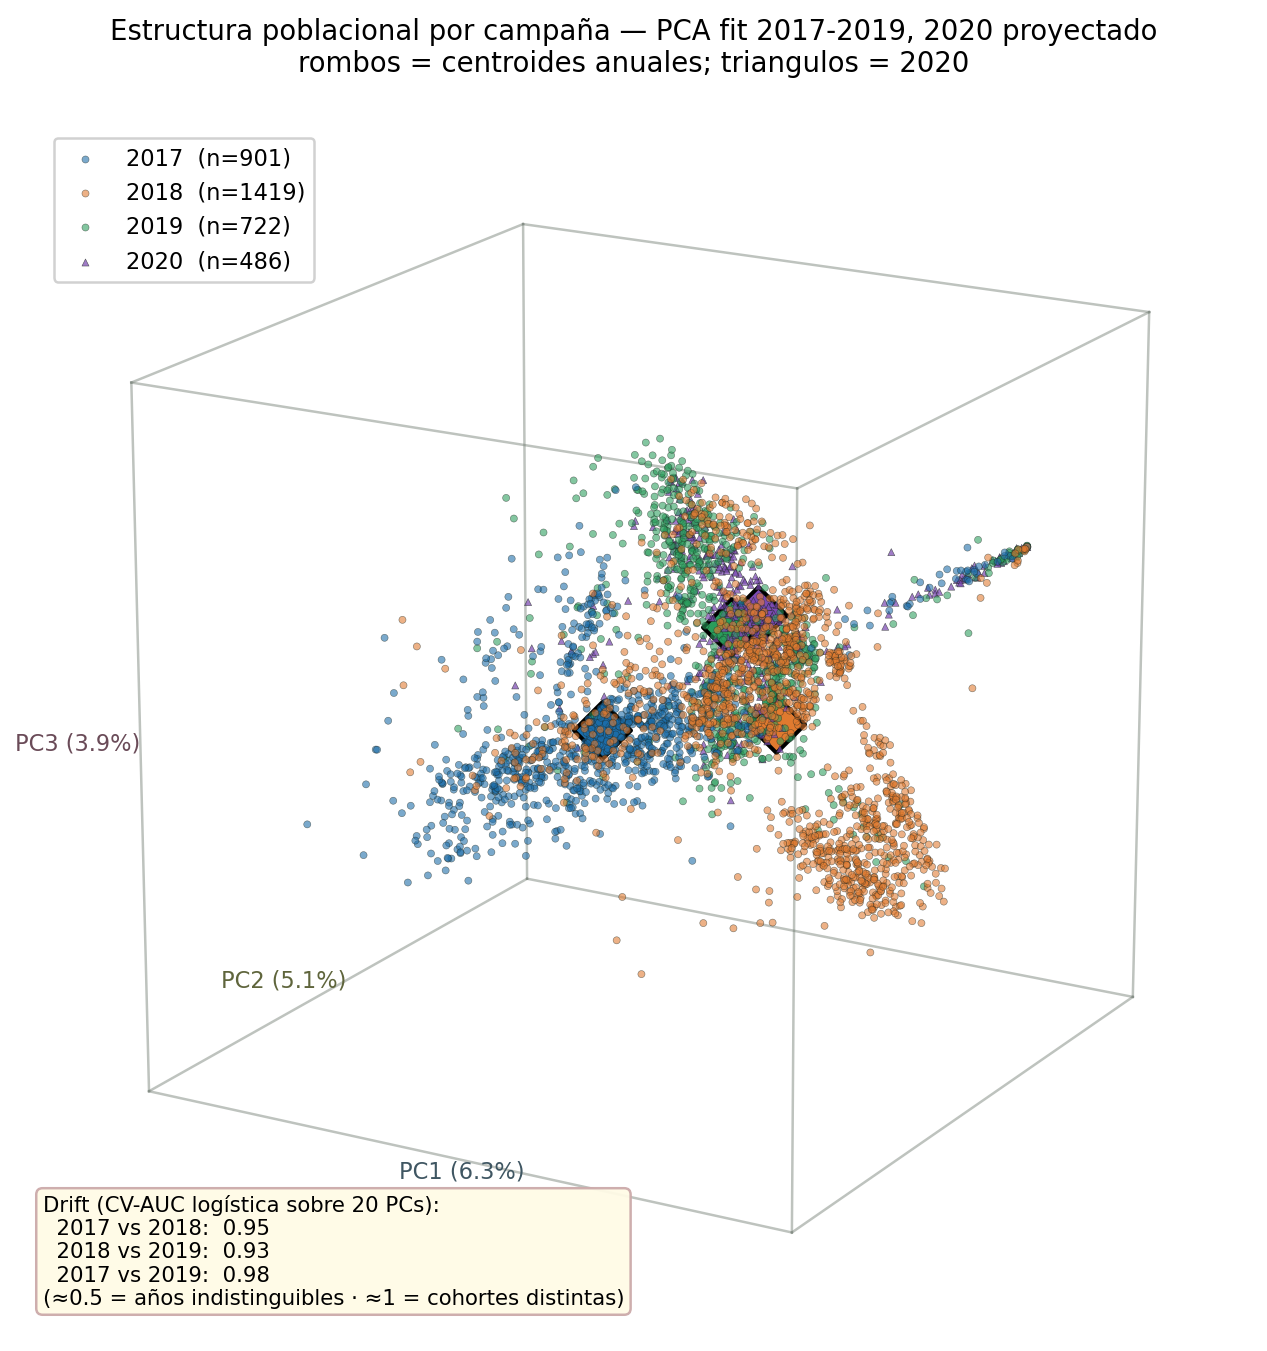
\includegraphics[width=0.99\columnwidth]{fig_eda_drift.png}
\caption{Estructura poblacional (PCA de SNPs) por campaña sobre el conjunto de desarrollo, con $2020$ proyectado (triángulos). Los centroides anuales se separan y la separabilidad genética (AUC $0.93$--$0.98$) confirma la deriva temporal que motiva un \textit{split} temporal.}
\label{fig:drift}
\end{figure}

\section{Metodología}
\subsection{Baseline de industria: GBLUP}
GBLUP (\textit{Genomic Best Linear Unbiased Prediction}) es el modelo mixto lineal estándar de la selección genómica \cite{vanraden2008}. Modela el fenotipo como $\mathbf{y}=\mathbf{1}\mu+\mathbf{g}+\boldsymbol{\varepsilon}$, donde $\mathbf{g}\sim\mathcal{N}(\mathbf{0},\,\sigma_g^2\mathbf{G})$ es el valor genético (el mérito heredable de la línea) y $\mathbf{G}$ es la matriz de parentesco genómico de VanRaden, $\mathbf{G}=\mathbf{Z}\mathbf{Z}^\top/p$, con $\mathbf{Z}$ la matriz de marcadores centrada. La predicción BLUP es
\begin{equation}
\hat{\mathbf{g}} = \mathbf{G}\big(\mathbf{G}+\lambda\mathbf{I}\big)^{-1}(\mathbf{y}-\mathbf{1}\hat\mu),\qquad \lambda=\sigma_\varepsilon^2/\sigma_g^2 ,
\end{equation}
y es equivalente a una regresión \textit{ridge} sobre los marcadores \cite{murphy2022}: cada SNP recibe un efecto pequeño y encogido, hipótesis \textit{infinitesimal} que ajusta adecuadamente a caracteres poligénicos como el rendimiento. Los componentes de varianza $\sigma_g^2,\sigma_\varepsilon^2$ se estiman por máxima verosimilitud restringida (REML). GBLUP constituye el estándar por carecer de hiperparámetros que ajustar (el \textit{shrinkage} se deriva de los propios datos), ser determinista, escalar a decenas de miles de marcadores y capturar de forma óptima la señal aditiva, que domina la heredabilidad —la fracción de la varianza fenotípica atribuible a causas genéticas— de la mayoría de los caracteres agronómicos.

\subsection{Baselines de contraste}
Para verificar que las mejoras posteriores no son triviales, se contrasta GBLUP con modelos no lineales estándar. Un \textbf{gradient boosting} de árboles (XGBoost \cite{chen2016}) y un \textbf{perceptrón multicapa} (MLP) alimentado con los SNPs sin transformar alcanzan, en el rendimiento óptimo de $2019$, un Pearson de $0.216$ y $0.291$ respectivamente, ambos por debajo del $0.315$ de GBLUP: capturar interacciones o no-linealidades genéricas no compensa el sobreajuste en $p\gg n$. La reducción de dimensionalidad tampoco aporta: precomprimir los SNPs con PCA antes de GBLUP no supera al baseline —a lo sumo lo iguala, dado que el \textit{kernel} $\mathbf{G}=\mathbf{Z}\mathbf{Z}^\top/p$ ya emplea toda la información y la rotación de PCA resulta redundante—, y XGBoost sobre latentes de PCA o de autoencoder queda igualmente por debajo. Se concluye que la mejora requiere explotar la estructura del problema y no cambiar de familia genérica.

\subsection{Red neuronal multitarea}
El análisis exploratorio sugiere que compartir la representación entre caracteres correlacionados puede tener un efecto regularizador. Una red \textbf{multitarea} de tronco compartido, con una cabeza lineal por combinación carácter$\times$ambiente (un \textit{ensemble} de varias semillas, sin ruteo), constituye el primer paso más allá de una red por objetivo. Predecir conjuntamente los seis fenotipos iguala a GBLUP en el rendimiento óptimo ($0.318$) y lo supera de forma moderada en sequía, lo que confirma que el aprendizaje multitarea es una palanca útil y motiva el desarrollo posterior.

\subsection{Mixture-of-Experts ruteado por subpoblación}
La contribución central de este trabajo parte de una hipótesis sobre cómo aprovechar los datos multigeneracionales. El entrenamiento reúne tres campañas con deriva entre sí, de modo que una red global las promedia y diluye la información específica de cada subpoblación, mientras que la deriva penaliza el uso indiscriminado del histórico. La hipótesis es que ese histórico \emph{sí} puede aprovecharse si se lo agrupa de forma coherente: agrupar las líneas por subpoblación genómica permite que cada predictor aprenda de las líneas emparentadas que le son relevantes, con independencia de la generación. Esta idea se relaciona con los \textit{Sparse Selection Indices} de López-Cruz \textit{et al.}\ \cite{lopezcruz2021}. Un índice de selección predice el mérito de una línea como combinación lineal de la información genómica disponible; su variante \textit{sparse} introduce esparsidad, seleccionando para cada predicción únicamente los individuos de entrenamiento más informativos —en general, los más emparentados con el objetivo— y descartando el resto, lo que en un contexto multigeneracional evita que campañas lejanas y poco relacionadas contaminen la predicción. El modelo propuesto traslada esa intuición a un régimen no lineal y la implementa de forma dura: en lugar de seleccionar un subconjunto por objetivo, particiona el panel en subpoblaciones y entrena un experto especializado en cada una.

Se propone así un \textbf{Mixture-of-Experts (MoE)} multitarea, esquematizado en la Fig.~\ref{fig:moe}, estructurado en dos etapas. La primera, de \emph{caracterización de subpoblaciones}, reduce la dimensionalidad de los SNPs con PCA ($100$ componentes) y agrupa el espacio latente con un modelo de mezcla gaussiana (GMM, $k=4$); el uso de una reducción lineal se apoya en que la estructura poblacional está codificada linealmente en los marcadores (Sec.~II). La segunda, de \emph{predicción de fenotipo}, rutea cada muestra de forma \textbf{dura} (\textit{hard top-1}) al experto de su cluster de mayor responsabilidad, que produce la predicción. Cabe destacar que el ruteo opera sobre el espacio comprimido mientras que los expertos reciben los \textbf{SNPs completos}: la PCA y el GMM solo determinan \emph{qué} experto responde, no \emph{con qué} información predice.

Cada experto es, a su vez, una red \textbf{multitarea de seis cabezas} (GY, PH, AD $\times$ óptimo, sequía) ensamblada sobre cinco semillas, con tronco compartido, \textit{dropout} y pérdida de Pearson \cite{bishop2024}. Dado que la partición de $n\approx2300$ muestras en cuatro clusters deja a cada experto con un número reducido de observaciones en pleno $p\gg n$, se incorporan dos salvaguardas: un tamaño mínimo de cluster (los clusters pequeños no entrenan un experto propio) y un \textbf{experto global de respaldo}, entrenado sobre la totalidad del conjunto, que atiende a los clusters pequeños o vacíos durante la inferencia. En el fold de reporte, los cuatro clusters reúnen $192/465/1265/398$ líneas y el de $192$ queda por debajo del umbral, de modo que operan tres expertos más el de respaldo.

\emph{Fundamento.} Los expertos por cluster disponen de un número reducido de observaciones, por lo que las cabezas auxiliares (PH, AD) actúan como una regularización que amplifica la ventaja del ruteo; a su vez, el tronco compartido \emph{entre ambientes} permite que la predicción en sequía aproveche la información del ambiente óptimo, de aprendizaje más sencillo. La combinación de estructura de subpoblación (ruteo) y de \textit{sharing} multitarea (expertos) es la que eleva la señal en el ambiente difícil, según reflejan los resultados.

\begin{figure}[!t]
\centering
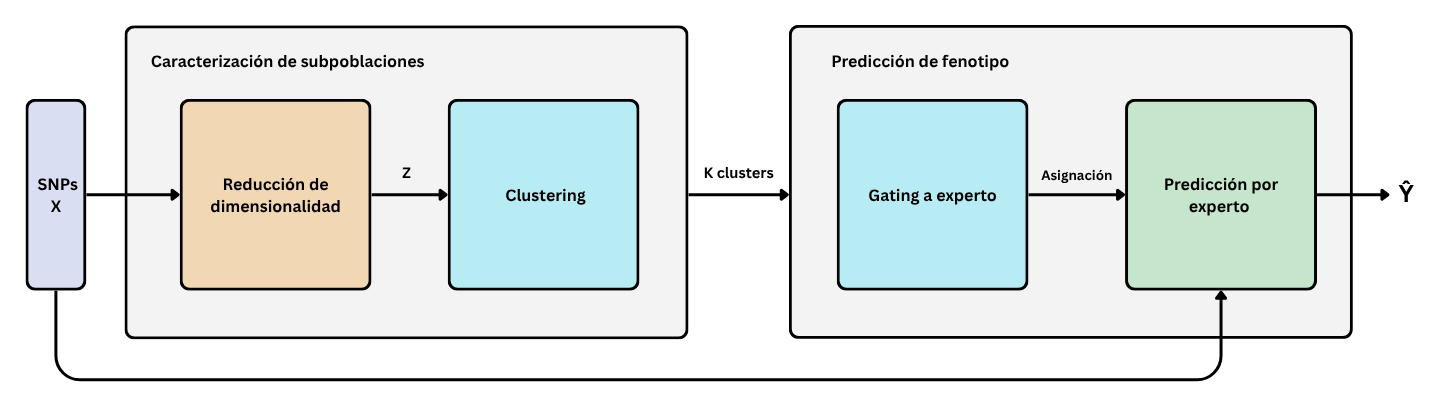
\includegraphics[width=\columnwidth]{fig_moe_diagram.png}
\caption{Arquitectura del Mixture-of-Experts. Los SNPs se reducen y agrupan para caracterizar la subpoblación (izquierda); el ruteo asigna cada línea a un experto que predice el fenotipo a partir de los SNPs completos (derecha).}
\label{fig:moe}
\end{figure}

\subsection{Variantes de ruteo}\label{sec:variantes}
El espacio de ruteo codifica un supuesto sobre qué criterio separa mejor a las líneas. Se estudian tres alternativas que atacan supuestos distintos. El \textbf{MoE soft}, inspirado en las mezclas suaves de expertos \cite{puigcerver2023} (no abordadas en clase), cuestiona el supuesto de que cada línea deba asignarse a una única subpoblación: reemplaza el ruteo duro por una combinación ponderada de expertos según las responsabilidades $r_k(\mathbf{x})$ del GMM, $\hat{y}(\mathbf{x})=\sum_k r_k(\mathbf{x})\,f_k(\mathbf{x})$. Al promediar, sin embargo, diluye la señal de subpoblación y alcanza un desempeño intermedio.

El \textbf{MoE PLS} cuestiona el supuesto de que el ruteo deba ser \emph{no supervisado}. La PCA maximiza la varianza de los marcadores, que recupera la ancestría pero es agnóstica al fenotipo; el ruteo por mínimos cuadrados parciales (PLS) busca en cambio direcciones $\mathbf{w}_k,\mathbf{c}_k$ que maximizan la covarianza entre marcadores y fenotipo,
\begin{equation}
\max_{\mathbf{w}_k,\mathbf{c}_k}\ \operatorname{Cov}\!\big(\mathbf{X}\mathbf{w}_k,\,\mathbf{Y}\mathbf{c}_k\big)\quad\text{s.a. }\|\mathbf{w}_k\|=\|\mathbf{c}_k\|=1 ,
\end{equation}
cuya primera dirección se alinea con la covarianza cruzada $\mathbf{X}^\top\mathbf{Y}$. El ruteo agrupa así por potencial fenotípico (vigor) en lugar de por ancestría, lo que beneficia al ambiente óptimo —donde el eje de vigor domina— y perjudica a la sequía, cuyo eje relevante (tolerancia al estrés) está débilmente alineado con el vigor general.

El \textbf{MoE GxE} cuestiona el supuesto de \emph{invariancia al ambiente}, esto es, que una misma partición y expertos compartidos sirvan para los dos ambientes. Ataca directamente la interacción genotipo-ambiente ($r=0.14$) aumentando el vector de ruteo con el indicador de ambiente, $\mathbf{z}'=[\mathbf{z};\,\gamma\,\mathbf{e}]$, y agrupando los pares (línea, ambiente): las columnas de óptimo y de sequía de una misma línea pueden así rutearse a expertos distintos. La corrección identifica correctamente que los ambientes difieren, pero, al separarlos por completo, elimina la transferencia por la que la sequía —con menos datos— tomaba fuerza del óptimo a través de un experto común; el remedio sobreactúa y degrada el ambiente difícil. El patrón resultante es sistemático: el ruteo \emph{no supervisado} (PCA) captura la estructura poblacional que beneficia a la sequía, mientras que todo ruteo \emph{supervisado o por ambiente} reorienta el modelo hacia el ambiente fácil.

\subsection{Alternativas descartadas}
Predecir el \textbf{residuo de GBLUP} con los expertos (descomponer $\mathbf{y}=\hat{\mathbf{g}}+\text{residuo}$) supera al baseline pero no alcanza al MoE directo ($0.32$ frente a $0.41$ en sequía), dado que la descomposición implica una pérdida de señal. El uso del latente de un \textbf{autoencoder} o de un \textbf{$\beta$-VAE} como espacio de agrupamiento, en lugar de PCA, se evaluó de forma preliminar sin resultados prometedores, en coherencia con la linealidad de la estructura poblacional, por lo que no se prosiguió. La sustitución de cada experto multitarea por uno \textbf{de una sola tarea} provoca un colapso del desempeño (cada experto observa un número reducido de líneas de un único ambiente y sobreajusta), lo que confirma que el \textit{sharing} multitarea resulta esencial. La poda de marcadores por desequilibrio de ligamiento —la correlación entre marcadores próximos que tienden a heredarse en bloque— previa al ruteo también deteriora el desempeño, dado que en un panel de mejoramiento esa redundancia constituye la estructura poblacional que el ruteo requiere.

\section{Experimentos, resultados y discusión}\label{sec:resultados}
\subsection{Protocolo e hiperparámetros}
Todos los modelos se evalúan sobre el \textbf{fold temporal fijo} (entrenamiento $2017$--$2018$, validación $2019$), con líneas disjuntas garantizadas. Los hiperparámetros de las redes y del ruteo se seleccionaron mediante \textbf{sweeps bayesianos} (Weights \& Biases) que optimizan el Pearson sobre un \textit{inner-split} temporal ($2017\rightarrow2018$), sin acceder a $2019$; el número de épocas se trata como un hiperparámetro adicional, seleccionado por Pearson de validación interna. GBLUP carece de hiperparámetros: su \textit{shrinkage} se deriva de REML. La incertidumbre de cada métrica se estima por \textbf{bootstrap con \textit{cluster} a nivel línea} ($2000$ remuestreos) y las comparaciones contra GBLUP emplean un bootstrap \emph{pareado} (mismo remuestreo para ambos modelos). Las redes se implementaron en PyTorch \cite{paszke2019}, mientras que la reducción de dimensionalidad, el agrupamiento y las líneas de base clásicas emplean scikit-learn \cite{pedregosa2011}.

\subsection{Resultados en validación (2019)}
La Tabla~\ref{tab:val2019} y la Fig.~\ref{fig:val2019} resumen la comparación para el rendimiento en ambos ambientes. En sequía —el ambiente más difícil y de mayor interés—, el MoE hard alcanza un Pearson de $0.407$ frente al $0.241$ de GBLUP (una diferencia de $+0.166$); el intervalo del $95\,\%$ del $\Delta$ pareado no incluye el cero, por lo que la mejora es estadísticamente significativa, y es la mayor registrada. Un análisis de ablación confirma que el aporte del ruteo no se explica solo por el ensamblado: el MoE supera de forma significativa al \textit{ensemble} global con idénticos hiperparámetros y semillas ($\Delta=+0.061$, IC$_{95}=[+0.015,+0.106]$). La misma jerarquía se observa en el \textit{matching20}, que asciende de $0.354$ (GBLUP) a $0.521$ (MoE hard): el modelo recupera cerca de la mitad del mejor $20\,\%$ de líneas por rendimiento.

En el ambiente óptimo el ordenamiento se invierte: los ruteos orientados al fenotipo —MoE GxE ($0.385$) y MoE PLS ($0.350$)— superan a GBLUP ($0.315$), mientras que el MoE hard, especializado en sequía, queda por debajo. Esta inversión es la manifestación directa de la interacción genotipo-ambiente descrita en la Sec.~II: no se observa un modelo uniformemente superior, sino que la arquitectura de mejor desempeño depende del ambiente. El MoE soft ocupa una posición intermedia en ambos ambientes, en coherencia con que el relajamiento del ruteo diluye la especialización.

\begin{table}[!t]
\renewcommand{\arraystretch}{1.2}
\caption{Pearson y \textit{matching20} (m20) predicho--observado en validación $2019$. m20 $=$ coincidencia del $20\,\%$ superior de líneas (azar $=0.20$). En negrita, el mejor por columna; los intervalos de confianza del Pearson se muestran en la Fig.~\ref{fig:val2019}.}
\label{tab:val2019}
\centering
\footnotesize
\begin{tabular}{lcccc}
\toprule
 & \multicolumn{2}{c}{\textbf{GY sequía}} & \multicolumn{2}{c}{\textbf{GY óptimo}} \\
\cmidrule(lr){2-3}\cmidrule(lr){4-5}
\textbf{Modelo} & Pearson & m20 & Pearson & m20 \\
\midrule
MoE hard        & \textbf{0.407} & \textbf{0.521} & 0.216 & 0.319 \\
MoE soft        & 0.291 & 0.403 & 0.279 & 0.368 \\
Red multitarea  & 0.275 & 0.368 & 0.318 & 0.389 \\
GBLUP           & 0.241 & 0.354 & 0.315 & 0.396 \\
MoE PLS         & 0.160 & 0.292 & 0.350 & \textbf{0.431} \\
MoE GxE         & 0.145 & 0.250 & \textbf{0.385} & 0.403 \\
\bottomrule
\end{tabular}
\end{table}

\begin{figure}[!t]
\centering
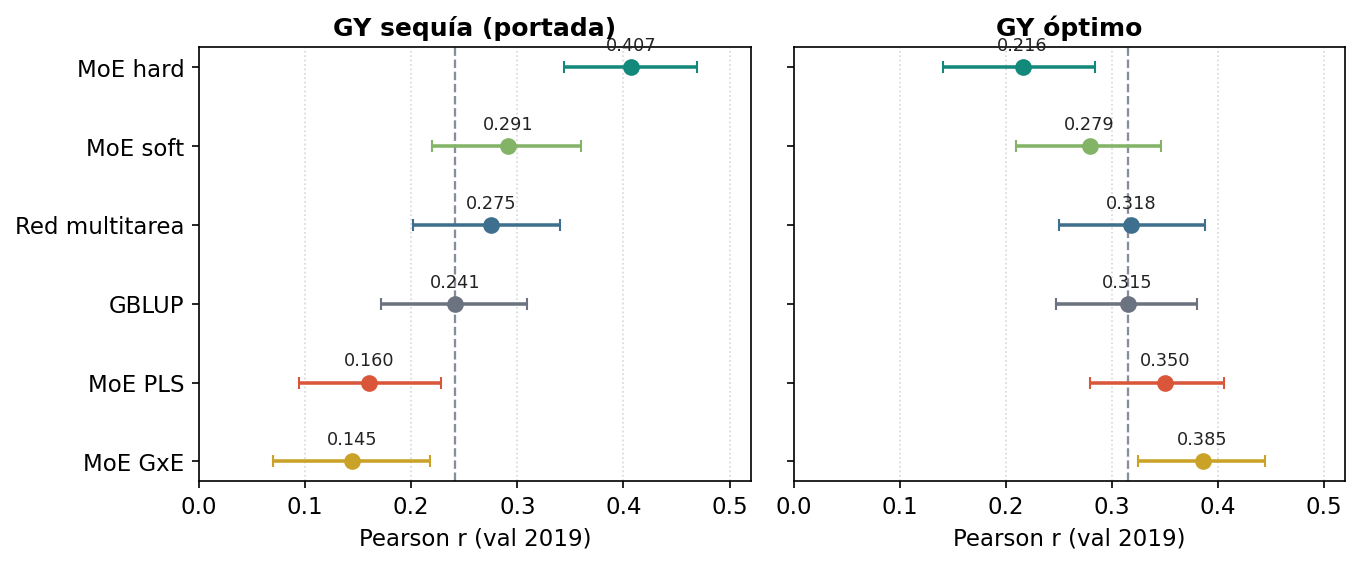
\includegraphics[width=\columnwidth]{fig_val2019.png}
\caption{Comparativa de modelos en validación $2019$ (Pearson $\pm$ IC$_{95}$; línea punteada $=$ GBLUP). En sequía el MoE hard domina; en óptimo el orden se invierte hacia los ruteos supervisados (GxE, PLS).}
\label{fig:val2019}
\end{figure}

\subsection{Resultados en test (2020)}
El criterio final de evaluación es la campaña $2020$, un ciclo nuevo sin solapamiento de líneas con el conjunto de desarrollo. Dado que la deriva penaliza a las campañas más antiguas, el entrenamiento se restringe a los \textbf{dos años más próximos al test ($2018$--$2019$)} en lugar de a todo el histórico. Aun así, la predicción de $2020$ a partir del genotipo colapsa para todos los modelos (Pearson nulo o negativo): en ausencia de líneas del ciclo objetivo no existe transferencia (\textit{cold-start}), y el $0.41$ obtenido en desarrollo no se sostiene al cruzar de ciclo. El resultado sugiere que, en este panel, la deriva temporal es un factor dominante y que la predicción genómica \emph{cross-cycle} pura del rendimiento tiene un margen limitado.

Una alternativa práctica es el \textbf{\textit{spike-in}}: fenotipar a campo una fracción reducida de líneas del ciclo nuevo, incorporarlas al entrenamiento y predecir las restantes. El fundamento de esta estrategia reside en la asimetría de costos del mejoramiento: genotipar una línea es económico y masivo, mientras que fenotipar su rendimiento exige cultivarla a campo durante una campaña completa, el paso más costoso y lento del proceso. Que baste con fenotipar un $5$--$10\,\%$ de las líneas de un ciclo nuevo para predecir con calidad el rendimiento del resto implica que un programa podría ensayar a campo solo una porción reducida de sus candidatos y estimar genómicamente la mayoría, con un ahorro considerable de superficie y de tiempo. La Tabla~\ref{tab:test2020} y la Fig.~\ref{fig:test2020} muestran que con un $5\,\%$ de líneas de $2020$ el signo se invierte para todos los modelos, y que con un $10\,\%$ los modelos de la familia MoE alcanzan un Pearson de hasta $0.50$ en sequía, frente al $0.34$ de GBLUP; la mayor parte del rescate se obtiene ya con ese primer $5\,\%$ (rendimiento marginal decreciente). En el ambiente óptimo el rescate es más homogéneo y GBLUP se mantiene competitivo, en coherencia con que la señal aditiva es su ámbito de mayor eficacia. Estos valores sugieren que un número reducido de observaciones del ciclo objetivo habilita la predicción genómica y que, en ese escenario, el MoE aprovecha esa información de forma más eficiente que el baseline aditivo.

\begin{table}[!t]
\renewcommand{\arraystretch}{1.2}
\caption{Cierre $2020$ con \textit{spike-in} (entrenamiento $2018$--$2019$ $+$ fracción de líneas de $2020$). Pearson sobre el $2020$ retenido, media de $3$ repeticiones. En negrita, el mejor por columna con \textit{spike}.}
\label{tab:test2020}
\centering
\footnotesize
\begin{tabular}{lccc}
\toprule
\textbf{Modelo (GY sequía)} & \textbf{0\,\%} & \textbf{5\,\%} & \textbf{10\,\%} \\
\midrule
MoE PLS        & $-0.059$ & $\mathbf{0.404}$ & $\mathbf{0.503}$ \\
MoE GxE        & $-0.038$ & $0.254$ & $0.493$ \\
Red multitarea & $-0.047$ & $0.316$ & $0.453$ \\
MoE soft       & $-0.109$ & $0.316$ & $0.452$ \\
MoE hard       & $-0.076$ & $0.254$ & $0.370$ \\
GBLUP          & $-0.143$ & $0.190$ & $0.338$ \\
\bottomrule
\end{tabular}
\end{table}

\begin{figure}[!t]
\centering
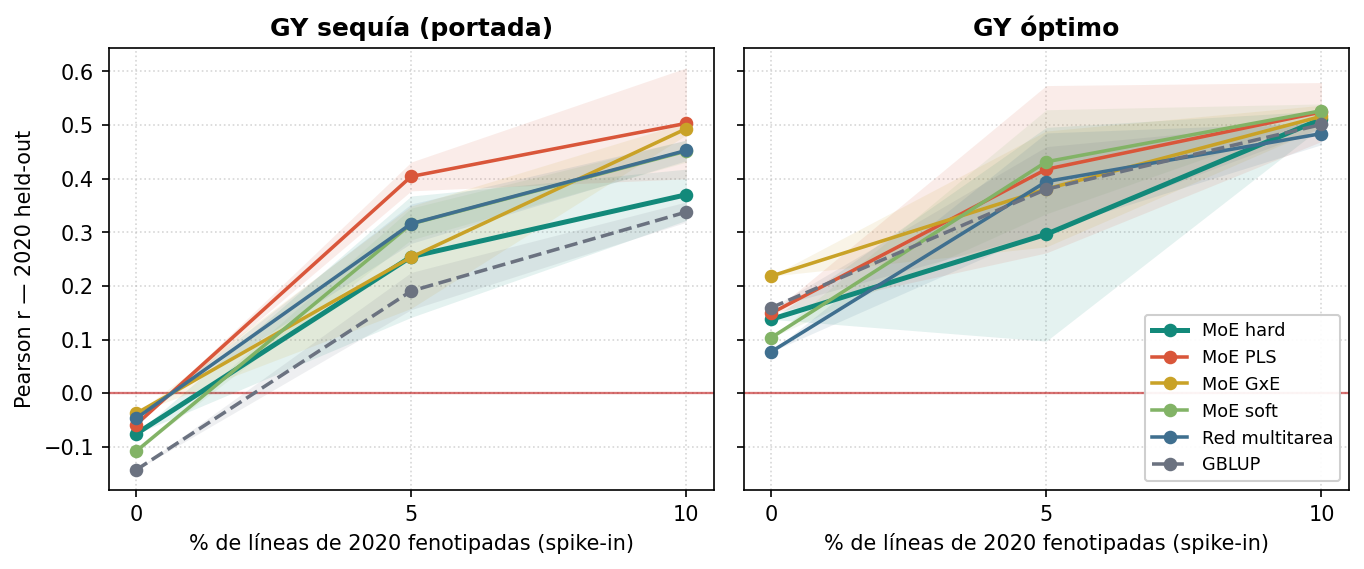
\includegraphics[width=\columnwidth]{fig_test2020.png}
\caption{Cierre $2020$: sin \textit{spike} todos los modelos colapsan (Pearson $\le 0$); con $5$--$10\,\%$ de líneas del ciclo nuevo la predicción se recupera y los modelos de la familia MoE superan a GBLUP.}
\label{fig:test2020}
\end{figure}

\subsection{Robustez al ruido y sobreajuste}
Dado que los SNPs pueden presentar error de genotipado, se mide la degradación del desempeño bajo un \textit{flip} Bernoulli de bits con probabilidad $\varepsilon$ (Fig.~\ref{fig:noise}). En sequía, el MoE hard es el más robusto en términos absolutos: retiene el $86\,\%$ de su Pearson a $\varepsilon=0.10$ ($0.407\rightarrow0.352$) y permanece por encima del resto en toda la curva. Los ruteos supervisados resultan frágiles (el MoE PLS retiene el $43\,\%$), ya que la perturbación de los marcadores altera su ruteo aprendido; GBLUP se mantiene estable pero en un nivel bajo. Que la ventaja del MoE persista bajo ruido sugiere que no se trata de un artefacto de datos limpios. Cabe señalar que el entrenamiento con ruido no mejora el desempeño: la robustez del MoE proviene de su regularización (\textit{dropout} y multitarea) y no de un \textit{data augmentation}.

Respecto del sobreajuste, inherente al régimen $p\gg n$, este se mitiga mediante la selección temporal de épocas e hiperparámetros, el \textit{shrinkage}/\textit{dropout}, el ensamblado de semillas y el \textit{sharing} multitarea que regulariza a los expertos. La concordancia entre el Pearson y el \textit{matching20} en la Tabla~\ref{tab:val2019} —el MoE hard lidera ambos en sequía— sugiere que la ventaja se asocia a una recuperación del ordenamiento de las líneas y no a un ajuste espurio de la escala.

\section{Conclusión y trabajo futuro}
Los resultados obtenidos indican que, en la validación temporal sobre este panel, un Mixture-of-Experts multitarea ruteado por subpoblación genómica mejora la predicción del rendimiento en sequía respecto de GBLUP, elevando la correlación de Pearson de $0.24$ a $0.41$, y que el aporte del ruteo persiste tras controlar por el efecto del ensamblado. El espacio de ruteo condiciona el ambiente favorecido y ningún modelo domina en ambos ambientes, lo que resulta coherente con la interacción genotipo-ambiente del conjunto; la elección de arquitectura queda, por tanto, sujeta al objetivo de mejoramiento. En el cierre sobre un ciclo enteramente nuevo, todos los modelos pierden capacidad predictiva a causa de la deriva temporal, y la incorporación de un $5$--$10\,\%$ de líneas fenotipadas del ciclo objetivo restablece las correlaciones, con una ventaja para los modelos propuestos frente al baseline aditivo. En conjunto, la evidencia apunta a que la ganancia proviene de explotar la estructura de subpoblación, más que de la capacidad no lineal por sí sola; su alcance fuera de este panel queda abierto a evaluación.

Como línea principal de trabajo futuro se propone reemplazar el agrupamiento discreto por un mecanismo de \textbf{atención} que capture las relaciones entre líneas de forma continua. El ruteo duro compromete cada línea a una única subpoblación; una capa de atención sobre el conjunto de entrenamiento permitiría ponderar de manera aprendida qué líneas son relevantes para predecir cada objetivo, como una generalización suave y diferenciable de la selección por parentesco que motivó el clustering. Cabría esperar que la atención modele relaciones línea--línea más finas que la partición del GMM, integre en un mismo modelo entrenable la caracterización de subpoblaciones y la predicción, y atenúe la sensibilidad de la asignación dura observada en el ruteo GxE.

\begin{thebibliography}{9}
\bibitem{lopezcruz2021} M. López-Cruz, Y. Beyene, M. Gowda, J. Crossa y P. Pérez-Rodríguez, ``Multi-generation genomic prediction of maize yield using parametric and non-parametric sparse selection indices,'' \textit{Heredity}, vol.~127, no.~5, pp.~423--432, 2021.
\bibitem{puigcerver2023} J. Puigcerver, C. Riquelme, B. Mustafa y N. Houlsby, ``From sparse to soft mixtures of experts,'' \textit{arXiv preprint} arXiv:2308.00951, 2023.
\bibitem{vanraden2008} P. M. VanRaden, ``Efficient methods to compute genomic relationship matrices,'' \textit{Journal of Dairy Science}, vol.~91, no.~11, pp.~4414--4423, 2008.
\bibitem{murphy2022} K. P. Murphy, \textit{Probabilistic Machine Learning: An Introduction}. MIT Press, 2022.
\bibitem{bishop2024} C. M. Bishop y H. Bishop, \textit{Deep Learning: Foundations and Concepts}. Springer, 2024.
\bibitem{price2006} A. L. Price, N. J. Patterson, R. M. Plenge, M. E. Weinblatt, N. A. Shadick y D. Reich, ``Principal components analysis corrects for stratification in genome-wide association studies,'' \textit{Nature Genetics}, vol.~38, no.~8, pp.~904--909, 2006.
\bibitem{chen2016} T. Chen y C. Guestrin, ``XGBoost: A scalable tree boosting system,'' en \textit{Proc.\ 22nd ACM SIGKDD}, 2016, pp.~785--794.
\bibitem{paszke2019} A. Paszke \textit{et al.}, ``PyTorch: An imperative style, high-performance deep learning library,'' en \textit{NeurIPS}, 2019.
\bibitem{pedregosa2011} F. Pedregosa \textit{et al.}, ``Scikit-learn: Machine learning in Python,'' \textit{JMLR}, vol.~12, pp.~2825--2830, 2011.
\end{thebibliography}

\end{document}
